\section{Secure Function Evaluation}
\label{sec:sfe-obdd}


For our protocols, we require a symmetric encryption scheme with two
easily attained special properties~\cite{LP04}, which are {\sf (1)} {\it elusive
range}: an encryption under one key is in the range of an encryption
with a different key with negligible probability, and {\sf (2)} {\it efficiently
verifiable range}: given a key, a user can efficiently verify that a
ciphertext is in the range of that key. These properties are required
so that the receiver of the garbled OBDD can correctly decrypt
nodes in the OBDD. The formal definition of these properties by
Lindell and Pinkas~\cite{LP04} is provided with the proofs. An example
of a symmetric key encryption scheme that fulfills these properties is
$E_k(m)=(r\,,\,f_k(r)\oplus m\,\|\,0^n)$, where
$f:\binset^n\times\binset^n\rightarrow\binset^{2n}$ is a pseudo-random
function and $r\rfrom\binset^n$ is a $n$-bit random sequence. Unless
stated otherwise, all symmetric key encryption schemes in this chapter,
besides being semantically secure (see section 2.?)
also require these two properties.  We will also use the $1$-out-of-$2$
oblivious transfer (denoted $OT^2_1$) protocol described in section 2.?.

We now give the protocol for securely computing an OBDD between two
parties where each party holds a part of the input. Assume $f$ is a
Boolean function $f(x_1,x_2,\cdots,x_n)$ of $n$ Boolean variables
$x_1,x_2,\cdots,x_n$. Let $OBDD(f)$ denote the OBDD for $f$ with the
ordering $x_1 < x_2 < \cdots < x_n$. We describe the protocol in stages.
Protocol 1 described in Section~\ref{sec:obdd-basicprotocol} assumes that
Alice holds inputs corresponding to the first $k$ variables, and 
Bob has the inputs corresponding to last $n-k$ variables
$x_{k+1},\ldots,x_n$. Protocol 2 described in Section~\ref{subsec:protocol2}
allows arbitrary sharing of inputs, and it uses the restriction
operation on OBDDs described earlier to reduce the bandwidth requirement
of the protocol.

\subsection{Protocol 1}
\label{sec:obdd-basicprotocol}


For this protocol, we assume that Alice holds the inputs
$(i_1,\ldots,i_k)$ corresponding to the first $k$ variables
$x_1,\ldots,x_k$, and Bob has the inputs $(i_{k+1},\ldots,i_n)$
corresponding to last $n-k$ variables $x_{k+1},\ldots,x_n$. In our
protocol, Alice and Bob want to compute $f(x_1,\cdots,x_n)$ on
their inputs using the OBDD for $f$. As the outcome, Bob learns
$f(i_1,\ldots,i_n)$.  This protocol is described in
Figure~\ref{protbasicobdd}.


\begin{figure*}

\begin{center}\begin{tabular}{cp{1in}c}
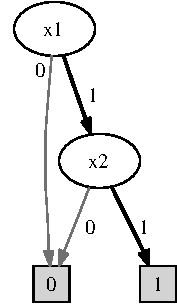
\includegraphics[%
    clip,
  scale=0.75]{obdd/figures/And1.pdf}&
&
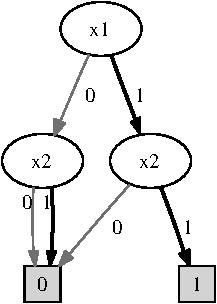
\includegraphics[%
  clip,
  scale=0.75]{obdd/figures/And1-full.pdf}\tabularnewline
Figure \ref{cap:BDDfill}(a)&
&
Figure \ref{cap:BDDfill}(b)\tabularnewline
\end{tabular}\end{center}
\caption{\label{cap:BDDfill}Adding dummy vertices}
\end{figure*}

One of the difficulties in developing and proving the protocol is
that OBDDs allow skipping of levels.  For example,
Figure~\ref{cap:BDDfill}(a) shows the OBDD for the Boolean function
$x_1 \wedge x_2$. Assume that the vertex at level $0$ is labeled with
$x_1$ and vertices at level $1$ are labeled with $x_2$. Suppose Alice
owns variable $x_1$ and Bob owns variable $x_2$. If Alice's input
is $1$, then Bob follows one more edge than if Alice's input were
$0$, which allows Bob to determine Alice's input. Compare this to
Figure~\ref{cap:BDDfill}(b), where a dummy vertex is added so
that, regardless of Alice's input, Bob has to follow the same number of
edges. In this case, Bob learns nothing about Alice's input. Before
Alice garbles the OBDDs, she adds dummy vertices so that each path
from the root to a terminal node has the same number of edges.  Alice adds
dummy nodes whenever $OBDD(f)$ allows Bob to skip levels when
evaluating the OBDD on his share of the input. Recall that the
$0$-successor and $1$-successor of $v$ is denoted by ${\it low}(v)$
and ${\it high}(v)$. For example, if node $n$ at level $j$ has node $n'''$ at level
$j+3$ as its $0$-successor, then Alice inserts two dummy nodes $n'$
and $n''$ at level $j+1$ and $j+2$ respectively. The $0$-successor of
node $n$ is changed to $n'$, both $0$ and $1$-successors of $n'$ are
set to $n''$, and both $0$ and $1$-successors of $n''$ are set to
$n'''$.

\vspace{2ex}
The steps of protocol 1 are as follows:

%\begin{center}
%\begin{boxfig*}{ht!}{
\textsc{\bf Input:} Both parties' inputs include the $OBDD(f)$ for the Boolean function
$f(x_1,x_2,\cdots,x_n)$ with the ordering $x_1 < x_2 < \cdots < x_n$.
Furthermore, Alice holds the inputs $(i_1,\ldots,i_k)$ corresponding
to the first $k$ variables $x_1,\ldots,x_k$, and Bob has the inputs
$(i_{k+1},\ldots,i_n)$. 
\vspace{1ex}
\begin{enumerate}
\item Alice performs the following steps:
\begin{enumerate}
\item She traverses the $OBDD(f)$ using her
input $(i_1,\cdots,i_k)$, which results in a node $v_{init}$ at level
$k$.

\item She uniformly and independently at random creates $(n-k)$ pairs
of secrets $(s_1^0,s_1^1),\cdots,(s_{n-k}^0,s_{n-k}^1)$.  In addition,
for each node $v$ in the $OBDD(f)$ whose level is between $k$ and $n-1$,
Alice also creates a secret $s_v$. 

\item She assigns a uniformly random label to each node whose level is
between $k$ and $n$. We refer to the randomly assigned label of node
$v$ using the notation $label(v)$.

\item Next, Alice augments $OBDD(f)$ with some number of dummy nodes
(to ensure that Bob always traverses $n-k$ nodes in his phase of the protocol). 


\item Alice garbles all nodes whose level is between $k$ and $n-1$
in the following manner. Let $v$ be a node in $OBDD(f)$ such $k \leq
{\it level}(v) \leq n-1$ and define ${\it level}(v)=\ell$. The encryption of node $v$, denoted
by $E^{(v)}$, is a label and a randomly ordered ciphertext pair
\[
\left(label(v)\,\,,\,\,E_{s_v \oplus s_{\ell-k+1}^0} (label(low(v)) \,\|\, s_{{\it low}(v)})\,\,\,,\,\,\,
E_{s_v \oplus s_{\ell-k+1}^1} (label(high(v)) \,\|\, s_{{\it high}(v)})\right)\,\,\,,
\]
where the labels are pre-pended to the secret with a separator symbol
and the order of the ciphertexts is determined by a fair coin
flip. Roughly speaking, the secrets corresponding to the $0$-successor
and $1$-successor of node $v$ are encrypted with the secret
corresponding to $v$ and its level.

Note that dummy nodes have the same structure as normal nodes, except
that the ciphertext pair contain encryptions of the same message since
dummy nodes have the same $0$ and $1$-successors. Provided the
encryption scheme is semantically secure, this poses no problem since
the keys are chosen uniformly at random.

Lastly, there are two terminal nodes of the form $(b,label(t_b))$ for
$b=0$ or $1$. Recall that $OBDD(f)$ has two terminal nodes, denoted as
$0$ and $1$, that are at level $n$.

\item Once Alice is done encrypting, she sends to Bob the encryption
of all nodes whose level is between $k$ and $n$ and the secret
$s_{v_{init}}$ corresponding to node $v_{init}$ at level $k$. We called
this the garbled OBDD.

\end{enumerate}

\item Bob performs the following steps:
\begin{enumerate}
\item He engages in $n-k$ 1-out-of-2 oblivious transfers to obtain the
secrets corresponding to his input. For example, if his input $i_j$ is
$0$, then he obtains the (level) secret $s_{j-k}^0$; otherwise, he
obtains the secret $s_{j-k}^1$.

\item Now Bob is ready to start his computation. Suppose
$i_{k+1}=0$. With $s_{1}^0$ and $s_{v_{init}}$, he decrypts both
ciphertexts in $E^{(v_{init})}$ and decides which gives the correct
result by using the verifiable range property of the encryption
scheme. Bob now has both $s_{{\it low}(v)}$ (the secret corresponding
to the $0$-successor of $v_{init}$) and $label(low(v))$ (which tells
Bob which encrypted node is used to evaluate his next
input). Continuing this way, Bob eventually obtains a label
corresponding to one of the terminal nodes, which determines the
result of the OBDD on the shared inputs. Bob sends this result to
Alice.
\end{enumerate}

\end{enumerate}
%}
%\vspace{-0.1cm}
%\caption{\label{protbasicobdd} Protocol 1.}
%\end{boxfig*}
%\end{center}

We prove correctness and security in the semi-honest threat model,
defined in section 2.1.  Claim~\ref{claim:protocol1correct}
proves that protocol 1 is
correct; that is, Bob computes the function $f(i_1,\cdots,i_n)$.
Claim~\ref{claim:protocol1secure} proves that protocol 1 is secure
in the semi-honest model; that is, at the end of protocol 1, Alice only
knows its input and the value of the function $f(i_1,\cdots,i_n)$, and
similarly for Bob. For our proofs, we require the definition of elusive range and
efficiently verifiable range from Lindell and Pinkas~\cite{LP04}.
\begin{definition}
Let \alg{(G},\alg{E},\alg{D)} be a symmetric key encryption scheme
with key-generation, encryption, and decryption algorithms.
Denote the range of the scheme by
$\alg{Range}_n(k)=\{E_k(x)\}_{x\in\binset^n}$. We say that
\begin{enumerate}
	\item \alg{(G},\alg{E},\alg{D)} has an \textbf{elusive range}
	if for every probabilistic poly-time machine A, every
	polynomial $p(\cdot)$, and all sufficiently large $n$,
	$\Pr_{k\from\alg{G(1^n)}}[A(1^n)\in\alg{Range}_n(k)]<1/p(n)$.

	\item \alg{(G},\alg{E},\alg{D)} has an \textbf{efficiently
	verifiable range} if there exists a prob. poly-time
	machine $M$ such that $M(1^n,k,c)=1$ if and only if
	$c\in\alg{Range}_n(k)$.
\end{enumerate}
\end{definition}

\begin{claim} If the encryption scheme has an elusive range and the
oblivious transfer protocol is secure, then Protocol 1 is correct for
semi-honest Alice and Bob.
\label{claim:protocol1correct}
\end{claim}
\begin{proof}
First we show that every node in the garbled OBDD sent to Bob can be
evaluated correctly. For an encrypted node $v$, let $c_0$ and $c_1$ be
the first and second ciphertext term. Suppose $k$ is the key that Bob
obtains to decrypt the ciphertext in node $v$. Because the
encryption scheme is elusive and all the keys used in the garbled OBDD
are chosen uniformly and independently at random, it follows
immediately that, except with negligible probability, only one
ciphertext in an encrypted node decrypts correctly; that is,
either $c_0\in\alg{Range(k)}$ or $c_1\in\alg{Range(k)}$ but not
both. Hence, except with negligible probability, every node in the
garbled OBDD can be evaluated correctly.

By induction, we show that the correct key is obtained for every node
input and output. The base case is the key $s_{v_{init}}$ and the 
keys $s^{i_{k+1}}_{k+1},\ldots,s^{i_{n}}_{n}$ (corresponding to Bob's
input) obtained from Alice through the $n-k$ oblivious transfers. The
inductive step at node $v$ assumes that the correct label (pointing
Bob to node $v$) and node key $s_v$ was obtained in the previous
step. Furthermore, the correct level key $s_l^{i_l}$ was obtained by
executing an oblivious transfer protocol. Since every node in the
garbled OBDD can be evaluated correctly and the garbled OBDD is built by
a semi-honest Alice, Bob obtains the correct label and key output at
node $v$, which concludes the inductive step. We can conclude that the
entire garbled OBDD can be evaluated to give the correct result.\footnote{
Note that the negligible probability of error during
decryption can be removed by Alice first checking that every encrypted
node decrypts correctly before sending the garbled OBDD to Bob.
}
\end{proof}



\begin{claim} If the encryption scheme is semantically secure and has an
efficiently verifiable elusive range, and the oblivious transfer
protocol is secure, then Protocol 1 is secure against semi-honest
Alice and Bob.
\label{claim:protocol1secure}
\end{claim}
\begin{proof} 

%[{\it Proof of Claim~\ref{claim:protocol1secure}}]

Intuitively, Bob's security follows directly from the security of the
1-out-of-2 oblivious transfer protocol he uses to obtain the secrets
corresponding to his input. Alice's security follows from both the
security of the oblivious transfer protocol (allowing Bob to only
obtain only one key per node) and the semantic security of the
encryption scheme (which allows Bob to only decrypt one entry in each
node). We now flesh out the details by providing a simulation proof
from Alice and Bob's view of the protocol. Let $x$ and $y$ be the
inputs of Alice and Bob respectively and $\Pi$ be a protocol for
secure-function evaluation of $f(x,y)$.  Let ${\sf VIEW}_A^\Pi (x,y)$
and ${\sf VIEW}_B^\Pi (x,y)$ be the view of Alice and Bob for the run
of the protocol $\Pi$ on input $x$ and $y$ (view of a party consists
of its input, output, and all messages it receives during the
execution of the protocol). In a simulation proof one needs to show
two probabilistic polynomial-time algorithms $S_A$ and $S_B$ such that
$S_A (x,f(x,y))$ and $S_B (y,f(x,y))$ are computationally
indistinguishable from ${\sf VIEW}_A^\Pi (x,y)$ and ${\sf VIEW}_B^\Pi
(x,y)$, respectively.  For a precise definition of a simulation proof
the reader should refer to~\cite[Chapter 7]{Goldreich:vol2}.

We first consider the case where Alice is corrupt. Alice's view in an
execution of Protocol 1 consists of her view of the oblivious transfer
protocol executions and the output of the function from Bob at the
end. We now build a simulator that simulates Alice's view given access
only to her input and output. Because the oblivious transfer protocol
is secure, there exists a simulator that can simulate the transcript
of Alice's view of the oblivious transfer protocol without knowing
Bob's input. On input $(i_1,\ldots,i_k, f(i_1,\ldots,i_n))$, the
simulator first simulates Alice's view of all $n-k$ executions of the
oblivious transfer protocol by repeatedly running the oblivious
transfer protocol simulator. Using a standard hybrid argument on the
transcripts of all $n-k$ executions oblivious transfer protocols, we
see that if the oblivious transfer protocol is secure, then the
distributions of the simulated and real combined transcripts of all
$n-k$ oblivious transfer executions are indistinguishable with
non-negligible probability.

Finally, the simulator writes $f(i_1,\ldots,i_n)$ on the transcript
of Alice's view. We now show that the distribution of the output $f$
is indistinguishable (except with negligible probability) from the
real output, which amounts to showing that Bob outputs
$f(i_1,\ldots,i_n))$ correctly on a real interaction. By the security
of the oblivious transfer protocol, Bob is provided with the correct
keys corresponding to its input during each execution of the oblivious
transfer protocol. Applying claim~\ref{claim:protocol1correct}, it
follows immediately that, except with negligible probability, Alice
obtains the correct output from Bob, except with negligible
probability. Therefore, the distribution of the simulated transcript
is indistinguishable, except with negligible probability, from a real
transcript, concluding the case when Alice is corrupt.

We now consider the case when Bob is corrupt. Given
$(i_{k+1},\ldots,i_n, f(i_1,\ldots,i_n))$, the simulator $\simu$ must
simulate both a garbled OBDD that Bob can use to correctly compute
$f(i_1,\ldots,i_n)$, and Bob's view of the $n-k$ executions of the
oblivious transfer protocol. We first show how $\simu$ simulates the
$n-k$ oblivious transfer protocol executions. As in the previous case,
because the oblivious transfer protocol is secure, there exists a
simulator that can simulate the transcript of Bob's view of the
oblivious transfer protocol without knowing Alice's input. Therefore,
$\simu$ simulates Bob's view of all $n-k$ executions of the
oblivious transfer protocol by running the oblivious transfer protocol
simulator $n-k$ times. Using a standard hybrid argument on the
transcripts of the oblivious transfer protocols, we see that if the
oblivious transfer protocol is secure, then the distributions of the
simulated and real transcripts of all $n-k$ oblivious transfer
executions are indistinguishable except with negligible probability.

We now show how $\simu$ builds a garbled OBDD that Bob can use to
successfully compute $f(i_1,\ldots,i_n)$. Since $\simu$ does not know
$i_1,\ldots,i_k$, it cannot generate the garbled OBDD according to the
protocol instructions. Instead, $\simu$ generates a garbled OBDD that
always evaluates to $f(i_1,\ldots,i_n)$ regardless of the keys
used. Such a garbled OBDD is built by first generating a chain of $n-k$
garbled nodes $n_{k+1},\ldots,n_{n}$ such that Bob's computation
starts at  $n_{k+1}$ and proceeds along the chain through
$n_{k+2}$ and so on, before ending at node $n_{n}$; note that there is
one such node for every level from $k+1$ to $n$. To ensure the
computation always proceeds along this chain, \textit{both}
ciphertexts in garbled nodes $n_{k+1},\ldots,n_{n-1}$ are encryptions
(under different keys) of the same label-key message such that the
label points to the next node along the chain and the node key
combined with the level key allows successful decryption of that node;
for example, simulated node $n_j$ for $k+1 \leq j\leq n-1$ has the
form
\[
\begin{array}{l}
\left( label(n_j)\,\,,\,\,E_{s_{n_j} \oplus s_{l}^0} (label(n_{j+1}) \,\|\, s_{n_{j+1}}) \right. \\
\left. E_{s_{n_j} \oplus s_{l}^1} (label(n_{j+1}) \,\|\, s_{n_{j+1}})\right)\,\,\,.
\end{array}
\]
Node $n_{n}$ is the terminal node and it is set to
$f(i_1,\ldots,i_n)$. Once $n_{k+1},\ldots,n_{n}$ is generated, the
simulator generates a number of ``fake'' nodes so that the simulated
garbled OBDD contains the correct number of nodes; this number can be
determined from $OBDD(f)$. Fake nodes are nodes whose ciphertext pair
contain encryptions under different keys of the same label-key
message; in a fake node, the label, the keys used to encrypt the
ciphertext pair, and the label-key message encrypted in the ciphertext
pair are chosen randomly.

All that remains is to show that the distribution of the simulated
garbled OBDD is indistinguishable from that of a real garbled OBDD. We
do this by using a standard hybrid argument over the nodes in the
garbled OBDD. Specifically, we run hybrid experiments with garbled OBDDs
where real nodes are replaced by simulated nodes. We define the hybrid
distributions such that $H_0(i_1,\ldots,i_n)$ contains the real
garbled OBDD and $H_{B}(i_1,\ldots,i_n)$ contains the simulated garbled
OBDD where $B$ is the number of non-dummy nodes in the real garbled
OBDD. We do not need to consider dummy nodes in our hybrid experiment
OBDDs because dummy nodes have the same distribution as the simulated
fake nodes and do not affect our argument.

We now define the hybrid garbled OBDD in experiment
$H_i(i_1,\ldots,i_n)$; the difficulty here is that the hybrid OBDD
contains both real and simulated nodes but must still allow Bob to
correctly compute $f(i_1,\ldots,i_n)$. First, we traverse the real
garbled OBDD and label a node as active if it is used by Bob in the
process of evaluating the OBDD and inactive otherwise. Note that there
will be only $n-k$ active nodes. Next, we order the nodes in the
garbled OBDD by their level with level $j+1$ nodes placed ahead of
level $j+2$ and so on; within the same level, nodes are ordered
arbitrarily. The hybrid OBDD is defined as follows: first take the real
garbled OBDD and replace the first $i$ non-dummy nodes as follows:
inactive nodes are replaced with simulated fake nodes. An active node
at level $j$ is altered by replacing its current ciphertext pair with
two encryptions of the label-key message corresponding to the next
active node at level $j+1$. These replacement ciphertexts are created
with the keys used to create the original ciphertext pair. Note that
the distribution of this altered active node is identical to that of
the simulated node $n_j$ in the node chain described above. It is easy
to see that a garbled OBDD built with this definition has the same
distribution as 1) a real garbled OBDD when $i=0$ (i.e. for $H_0$), and
2) a simulated garbled OBDD when $i=B$ (i.e. for $H_B$).

We are now ready to show that the distribution of the simulated
garbled OBDD is indistinguishable from that of a real garbled OBDD; that
is, we will show that
$\{H_0(i_1,\ldots,i_n)\}=\{H_{B}(i_1,\ldots,i_n)\}$. Suppose to the
contrary that the distributions are distinguishable; that is, there
exists a poly-time distinguisher $\disting$ that 
\[
\begin{array}{l}
\vert \Pr[\disting(H_0(i_1,\ldots,i_n))=1] - \\
\Pr[\disting(H_{B}(i_1,\ldots,i_n))=1]>1/p\vert
\end{array}
\]
 for some polynomial
$p$. Then there exists a $j$ such that 
\[
\begin{array}{l}
\vert
\Pr[\disting(H_{j-1}(i_1,\ldots,i_n))=1] - \\
\Pr[\disting(H_{j}(i_1,\ldots,i_n))=1]>1/pB\vert
\end{array}
\]

Using $\disting$, we now build an adversary that breaks the semantic
security of the encryption scheme used to encrypt the garbled
nodes. Recall in a semantic security game, the adversary sends two
messages $m_0,m_1$ to the challenger and receives the encryption of
$m_b$ for $b=\binset$; the adversary's goal is to determine $b$. Let
$n^j$ be the $j$th node and we denote its two ciphertext terms as
$c^{j}_0$ and $c^{j}_1$. Note that node $n^j$ in the hybrid OBDD in
distribution $H^*_{j-1}$ is a real garbled node, whereas the same node
for distribution $H^*_{j}$ is a simulated garbled node; specifically,
$c^{j}_0$ and $c^{j}_1$ in distribution $H^*_{j-1}$ are encryptions of
different label-key messages, whereas they are encryptions of the same
label-key message in distribution $H^*_{j}$. We exploit this fact to
build the adversary $\adver$ that breaks semantic security of the
encryption scheme.

First, $\adver$ creates the hybrid garbled OBDD corresponding to the
distribution $H^*_{j-1}(i_1,\ldots,i_n)$. One of the two ciphertexts
$c^{j}_0$ and $c^{j}_1$ in node $n^j$ is an encryption of the label
and key for the active node $n^{j+1}$, whereas the other ciphertext is
an encryption of the label and key for an inactive node. Let $\ell_0$
be the label-key message encrypted in $c^j_0$ and $\ell_1$ be that
encrypted in $c^j_1$. Next, $\adver$ sends $\ell_0$ and $\ell_1$ to
the semantic security challenger and receives $c^*$, which is an
encryption of either $\ell_0$ or $\ell_1$. Without loss of generality,
let $\ell_0$ be the label-key message (contained in ciphertext
$c^{j}_0$) that leads to the next active node. $\adver$ replaces
$c^j_1$ with $c^*$ in node $n^j$ in the garbled OBDD that it built in
the first step, and then feeds the altered OBDD together with the other
required inputs to the hybrid distinguisher $\disting$. Note that
$c^*$ cannot be decrypted with the node and level keys for node
$n^j$. This fact, however, does not prevent the garbled OBDD from being
evaluated correctly because $c^*$ replaces $c^j_1$, which contains the
label and key to an inactive node, and would not be successfully
decrypted while evaluating the garbled OBDD on the inputs
$(i_1,\ldots,i_n)$.

$\disting$ eventually outputs a result stating that the input is of
distribution $H^*_{j-1}$ or $H^*_{j}$. If $\disting$ outputs that the
input is of distribution $H^*_{j-1}$, then $\adver$ outputs that $c^*$
is an encryption of $\ell_1$; otherwise $\adver$ outputs that $c^*$ is
an encryption of $\ell_0$. Notice that if $c^*$ is an encryption of
$\ell_0$, then both ciphertexts in node $n^j$ are encryptions of the
same label-message, and the input to $\disting$ has distribution
$H^*_{j}$. Similarly, if $c^*$ is an encryption of $\ell_1$, then the
input to $\disting$ has distribution $H^*_{j-1}$. Since $\disting$
distinguishes between $H^*_{j-1}$ and $H^*_{j}$ with non-negligible
probability, we see that $\adver$ wins the semantic security game with
non-negligible advantage. Since we assume that the encryption scheme is
semantically secure, this implication is a contradiction, and there is
no such distinguisher $\disting$ that distinguishes between
$H_0(i_1,\ldots,i_n)$ and $H_{B}(i_1,\ldots,i_n)$; that is, the
distribution of the simulated garbled OBDD is indistinguishable from
that of a real garbled OBDD. Therefore, Bob's simulated view is
indistinguishable, except with negligible probability, to the real
view, concluding the proof.
\end{proof}



\subsection{Protocol 2}
\label{subsec:protocol2}

The protocol presented in this section allows both Alice and Bob to
possess arbitrary input sets instead of assuming that Alice (and also
Bob) holds either the first $k$ or the last $n-k$ input variables.  In
this new protocol, before garbling the OBDD, Alice can reduce the size
of the OBDD by eliminating vertices whose labels correspond to Alice's
inputs.  Let $f(x_1,\cdots,x_n)$ be the function to be computed and
$X_A$ denotes the inputs of Alice. Alice first computes the OBDD  for the restriction $f
\mid_{X_A}$ of $f$ for the variables in its input
set $X_A$. Alice then encrypts the reduced OBDD and sends it to
Bob. During the restriction operation, all vertices whose labels
correspond to Bob's input should be included. If this is not the case,
then there is a risk that different restrictions could produce
different numbers of nodes, which would leak information to Bob about
Alice's inputs. For example, in Figure~\ref{cap:BDDpe}(a), where
Alice's value is $0$, there are only 2 nodes, but in
Figure~\ref{cap:BDDpe}(b), there are 3 nodes.
Figure~\ref{cap:BDDpe}(c) shows the result of retaining extra
vertices, in which case there are 4 nodes regardless of Alice's
inputs. The description of this protocol is presented next.
The proof of correctness of this protocol
is almost identical to the one presented in
Section~\ref{sec:obdd-basicprotocol}. Example~\ref{example:protocol2} shows
an execution of this protocol on a small function.

\begin{figure*}

\begin{center}\begin{tabular}{cp{0.5in}p{1in}p{0.3in}c}
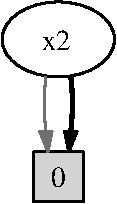
\includegraphics[%
  clip,
  scale=0.75]{obdd/figures/And1false.pdf}&
&
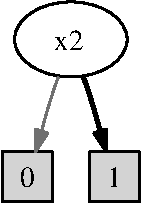
\includegraphics[%
  clip,
  scale=0.75]{obdd/figures/And1true.pdf}&
&
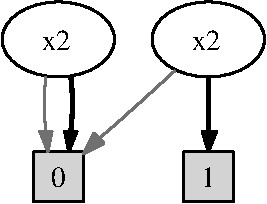
\includegraphics[%
  clip,
  scale=0.75]{obdd/figures/And1false2.pdf}\tabularnewline
Figure \ref{cap:BDDpe}(a)&
&
Figure \ref{cap:BDDpe}(b)&
&
Figure \ref{cap:BDDpe}(c)\tabularnewline
\end{tabular}\end{center}

\caption{\label{cap:BDDpe}OBDD restriction}

\end{figure*}

\vspace{2ex}
The steps of protocol 2 are as follows:

%\begin{center}
%\begin{boxfig}{ht!}{
\textsc{\bf Input:} Both parties' inputs include the $OBDD(f)$ for the Boolean function
$f(x_1,x_2,\cdots,x_n)$ with the ordering $x_1 < x_2 < \cdots < x_n$.
Furthermore, Alice holds the inputs for the variables in the set $X_A$ and
Bob holds the inputs for the variables in the set $X_B \; = \; \{ x_1,\cdots,x_n \} - X_A$.
\vspace{1ex}
\begin{enumerate}
\item Alice performs the following steps:
\begin{enumerate}
\item Alice computes the OBDD ${\cal O}_A$ for the function $f \mid_{X_A}$. This is the restriction
operation described in Section~\ref{sec:OBDDs}.

\item Alice encrypts the OBDD for the function $f \mid_{X_A}$ and sends it to Bob. This
step is exactly the same as for Protocol 1.  Alice also sends
the secret corresponding to the root of the OBDD ${\cal O}_A$. 


\end{enumerate}

\item The computation for Bob is exactly the same as that for Protocol 1. 

\end{enumerate}
%}
%\vspace{-0.1cm}
%\caption{\label{fig:protocol2} Protocol 2.}
%\end{boxfig}
%\end{center}


\begin{example}
\label{example:protocol2}
\rm Assume that Alice and Bob want to compute $f(x_1,x_2)  \; = \; x_1 \wedge x_2$, where
Alice has input $x_1$ and Bob has input $x_2$, or in other words $X_A
\; = \; \{ x_1 \}$ and $X_B \; = \; \{ x_2 \}$.  Assume that $x_1 = 0$
and $x_2 = 1$. $OBDD(f)$ with dummy nodes is shown in
figure~\ref{cap:BDDfill}(b). Alice computes the OBDD for the function
$f \mid_{ x_1 \leftarrow 0}$, which results in a structure shown in
Figure~\ref{cap:BDDpe}(c).  Let the two nonterminal nodes in
Figure~\ref{cap:BDDpe}(c) be $v_1$ and $v_2$. First, Alice generates
$2$ secrets $s_{v_1}$ and  $s_{v_2}$, which are assigned
to the nodes $v_1$ and $v_2$, respectively.   Alice also
generates random labels for the four nodes in
Figure~\ref{cap:BDDpe}(c), and  generates a pair of secrets
$(s_1^0,s_1^1)$. The garbled OBDD corresponding to
Figure~\ref{cap:BDDpe}(c) is shown below (terminal nodes
are shown as $0$ and $1$ and lab denotes label). 
\begin{center}
\begin{tabular}{|l|} \hline
$(lab(v_1), E_{s_{v_1} \oplus s_1^0} (lab(0)  \,\|\, s_0), E_{s_{v_1} \oplus s_1^1} (lab(0) \,\|\, s_0))$ \\ \hline
$(lab(v_2), E_{s_{v_2} \oplus s_1^0} (lab(0) \,\|\, s_0), E_{s_{v_2} \oplus s_1^1} (lab(1) \,\|\, s_1))$ \\ \hline
$(0,lab(0))$ \\ \hline
$(1,lab(1))$ \\ \hline
\end{tabular}
\end{center}
Alice reveals the secret $s_{v_1}$ corresponding node $v_1$.
Alice and Bob engage in a 1-out-of-2 ($OT^2_1$) protocol and Bob obtains the secret $s_1^1$ (recall that
$x_2 = 1$).
Bob can now decrypt the second component of the first entry of the garbled OBDD and
obtain $label(0) \,\|\, s_0$, and  Bob can infer that the output is $0$.
\end{example}

\begin{claim} If the encryption scheme has an elusive range and the
oblivious transfer protocol is secure, then Protocol 2 is correct for
semi-honest Alice and Bob.
\label{claim:protocol2correct}
\end{claim}
\begin{proof}
The proof of this claim is exactly same as the proof of Claim~\ref{claim:protocol1correct}.
One has to assume that the restriction operation used by Alice is correct.
\end{proof}

\begin{claim} If the encryption scheme is semantically secure and has an
efficiently verifiable elusive range, and the oblivious transfer
protocol is secure, then Protocol 2 is secure against semi-honest
Alice and Bob.
\label{claim:protocol2secure}
\end{claim}
\begin{proof}
%[{\it Proof Sketch for Claim~\ref{claim:protocol2secure}}]
The full proof is very similar for that in
Claim~\ref{claim:protocol1secure}, and we provide only a sketch. The
case when Alice is corrupt is identical to that in
Claim~\ref{claim:protocol1secure}. We briefly discuss why the proof is
also almost identical in the case when Bob is corrupt. The main
observation is that the simulator $\simu$ builds the simulated garbled
OBDD in the same way as in Claim~\ref{claim:protocol1secure} because
there is no difference in how Protocol 2 requires Bob to traverse the
garbled nodes given the same level keys. Therefore, the hybrid
distributions are defined the same way and the rest of the proof
follows.
\end{proof}

